

\documentclass{beamer}
%
% Choose how your presentation looks.
%
% For more themes, color themes and font themes, see:
% http://deic.uab.es/~iblanes/beamer_gallery/index_by_theme.html
%
\mode<presentation>
{
  \usetheme{default}      % or try Darmstadt, Madrid, Warsaw, ...
  \usecolortheme{default} % or try albatross, beaver, crane, ...
  \usefonttheme{default}  % or try serif, structurebold, ...
  \setbeamertemplate{navigation symbols}{}
  \setbeamertemplate{caption}[numbered]
} 

\AtBeginSection[]{%
\frame{
	
	\transsplitverticalin
	\frametitle{Outline}
	\tableofcontents[currentsection]
}
}

\usepackage[english]{babel}
\usepackage[utf8x]{inputenc}
\usepackage{amsmath}
\usepackage{booktabs}
\usepackage{longtable}

\newcommand\SmallerFont{\fontsize{8}{10}\selectfont}

\setbeamertemplate{bibliography item}[text]

\addtobeamertemplate{navigation symbols}{}{%
	\usebeamerfont{footline}%
	\usebeamercolor[fg]{footline}%
	\hspace{1em}%
	\insertframenumber/\inserttotalframenumber
}

\title[Your Short Title]{Bitcoin as an Asset}
\subtitle{Correlation and Portfolio Allocation}
\author{Samuele Vianello}
%\institute{Where You're From}
\date{February 19th}

\begin{document}

\begin{frame}
  \titlepage
\end{frame}

% Uncomment these lines for an automatically generated outline.
\begin{frame}{Outline}
  \tableofcontents
\end{frame}

%\section{Introduction}

%\begin{frame}{Introduction}
%
%\begin{itemize}
%  \item Your introduction goes here!
%  \item Use \texttt{itemize} to organize your main points.
%\end{itemize}
%
%\vskip 1cm

%\begin{block}{Examples}
%Some examples of commonly used commands and features are included, to help you get started.
%\end{block}
%
%\end{frame}
\section{Dataset}

\begin{frame}[allowframebreaks]{Dataset}
The dataset contains the prices of different assets from \textit{August 2010}  to \textit{October 2018}, all values downloaded from Bloomberg. 
\begin{enumerate}
	\item Stock indexes:
	\begin{itemize}
		\item S\&P500: American stock market index based on 500 large company with stock listed either on the NYSE or NASDAQ.
		\item EURO STOXX 50: equity index of eurozone stocks, covering 50 stocks from 11 eurozone countries.
		\item MSCI BRIC: market cap weighted index designed to measure the equity market performance across the emerging country indices of Brazil, Russia, India and China.
		\item NASDAQ: market cap weighted index including all NASDAQ tiers: Global Select, Global Market and Capital Market.
	\end{itemize}
	\item Bond indexes:
	\begin{itemize}
		\item BBG Pan European: Bloomberg Barclays Pan-European Aggregate Index that tracks fixed-rate, investment-grade securities issued in different European currencies.
		\item BBG Pan US: Bloomberg Barclays US Aggregate Bond Index, a benchmark that measures investment grade, US dollar-denominated, fixed-rate taxable bond market.
		\item BBG Pan EurAgg: similar to the Pan European but only considers securities issued in euros.
	\end{itemize} 
	\item Currencies:
	\begin{itemize}
		\item EUR/USD
		\item GBP/USD
		\item CHF/USD
		\item JPY/USD
	\end{itemize}
	\item Commodities:
	\begin{itemize}
		\item Gold: price of gold measured in USD/Oz.
		\item WTI: price of crude oil used as benchmark in oil pricing and as the underlying commodity in the NYMEX oil future contracts.
		\item Grain: S\&P GPSCI index that measures the performance of the grain commodity market.
		\item Metals: S\&P GSCI Industrial Metals index that measures the movements of industrial metal prices including aluminium, copper, zinc, nickel and lead.
	\end{itemize}
\end{enumerate}
\end{frame}


\section{Empirical Correlation}




\section{Model}

\subsection{Merton Model}

\begin{frame}{Original Merton Model (1976)}
Original Merton 1976 \cite{MERTON1976} model:
\begin{equation}
\label{merton_model}
    \frac{dS_t}{S_t} = \alpha dt + \sigma dW_t  + (Y_t-1)dN
\end{equation}

where 
\begin{itemize}
    \item $\alpha$ is the drift
    \item $\sigma$ is the diffusion coefficient
    \item $Y_t$ is a process modelling the intensity of the jumps
    \item $N(t)$ is the Poisson process driving the arrival of the jumps and has parameter $\lambda$
\end{itemize}

\end{frame}


\begin{frame}{Dynamics of the log-returns}
%%%%% add references to cont-tankov and martin
We can rewrite (\ref{merton_model}) in terms of the log-returns $X_t = log(S_t)$ and obtain:
\begin{equation}
    dX_t = (\alpha - \frac{\sigma^2}{2})dt + \sigma dW_t + \log (Y_t)
\end{equation}

that has as solution:
\begin{equation}
\label{merton_returns}
    X_t =X_0 +  \mu t + \sigma W_t + \sum_{k=1}^{N(t)} \eta_k
\end{equation}

where 
\begin{itemize}
    \item $X_0=log(S_0)$
    \item $\eta_k= \log(Y_k) = \log(Y_{t_k})$ and $t_k$ is the time when the $k^{th}$ Poisson shock from $N(t)$ happens.
    $\eta_k$ are distributed as Gaussians: $\eta \sim \mathcal{N}(\theta , \delta^2)$
    \item $N^{(j)}(t)$ are Poisson processes with parameters $\lambda_j$, which are independent of $\mathbf{W}_t$ and of one another
    \item $\mu = \alpha - \frac{\sigma^2}{2} $ for ease of notation
\end{itemize}

\end{frame}
%
%\begin{frame}{Discretized dynamics of log-returns}
%
%It is often useful when dealing with market data that are by nature discrete, to consider a \textit{discretized} version of (\ref{merton_returns}) in which the values are sampled at intervals of $\Delta t$ in $[0, T]$. We thus get that for $X_i = \log(\frac{S_{i+1}}{S_i})$:
%
%\begin{equation}
%\label{discrete_returns}
%    X_i =  \mu \Delta t + \sigma \sqrt{\Delta t} \; z +  \sum_{k=1}^{N_{i+1} - N_i} Y_k
%\end{equation}
%
%where we denote $X_i = X_{t_i}$, $N_i = N(t_i)$ and $t_i = i \Delta t$ with $i= 0 \dots N$, $t_N = N \Delta t= T$,  $z$ is distributed as a standard Gaussian $ z\sim \mathcal{N}(0,1)$.
%
% Following basic stochastic analysis, one can prove that the resulting value $N_{i+1} - N_i$,  is distributed as a Poisson random variable $N$ of parameter $\lambda \Delta t$.
%\end{frame}
%
%\begin{frame}{Original Merton Model (1976)}
%Applying the Total probability theorem, we get the following expression for the transition density:
%\begin{equation}
%\label{transitional}
%    f_{\Delta X} (x) = \sum_{k=0}^{\infty} \mathbb{P}(N = k) f_{\Delta X | N = k}(x) 
%\end{equation}
%
%This infinite mixture of Gaussian random variable makes the MLE intractable(see Honore). %%% add reference 
%To get a simpler definition of the log-return density, we limit our study to small values of $\lambda \Delta t$ so that the Poisson variable can only be in ${0,1}$ with non-negligible probability.
%\begin{equation*}
%\begin{split}
%    f_{\Delta X} (x) & = \mathbb{P}(N = 0) f_{\Delta X | N = 0}(x) + \mathbb{P}(N = 1) f_{\Delta X | N = 1}(x)\\
%             &= (1 - \lambda \Delta t) \;f_{\mathcal{N}}(x ; \mu, \sigma^2) + (\lambda \Delta t)\; f_{\mathcal{N}}(x ; \mu + \theta, \sigma^2+\delta^2)
%\end{split}
%\end{equation*}
%\end{frame}
%
%\begin{frame}{Multivariate Merton}
%Multivariate generalization of Merton's 1976 \textit{jump diffusion} for $n$ assets:
%\begin{equation}
%\label{merton_prices}
%    \frac{dS_t^{(j)}}{S_t^{(j)}} = \alpha_j dt + \sigma_j dW_t^{(j)} + (Y^{(j)}_t -1) dN^{(j)}_t
%\end{equation}
%
%where for $j = 1 ... n$ representing the assets:
%\begin{itemize}
%    \item $\mathbf{S}_t$ is the price vector
%    \item $\alpha_j$ are the drifts
%    \item $\sigma_j$ are the diffusion coefficients
%    \item $W^{(j)}_t$ are the components of an $n$-dimensional Wiener process $ \mathbf{W}_t$ with $dW^{(j)}dW^{(i)}=\rho_{j,i}$
%    \item $\eta_j$ represent the intensities of the jumps and are distributed as Gaussian: $\eta_j \sim \mathcal{N}(\theta_j , \delta_j^2)$
%    \item $N^{(j)}(t)$ are Poisson processes with parameters $\lambda_j$, which are independent of $\mathbf{W}_t$ and of one another
%\end{itemize}
%
%\end{frame}

%
%\begin{frame}{Multivariate transition density}
%We can proceed as in the univariate case in order to get an explicit formula for the transition density, conditioning on all the different Poisson processes. In the two asset case we have
%\begin{equation*}
%\begin{aligned}
%    f_{\Delta\mathbf{X}}(\mathbf{x}) &= \sum_{k_1=0}^{\infty}\sum_{k_2=0}^{\infty} \mathbb{P}(N^{(1)}(t) = k_1, N^{(2)}(t)=k_2) \\
%    &f_{\Delta\mathbf{X}}(\mathbf{x} | N^{(1)}(t) = k_1, N^{(2)}(t)=k_2)\\
%    &= \sum_{k_1=0}^{\infty}\sum_{k_2=0}^{\infty}\mathbb{P}(N^{(1)}(t) = k_1) \mathbb{P}(N^{(2)}(t)=k_2)\\
%    &f_{\Delta\mathbf{X}}(\mathbf{x} | N^{(1)}(t) = k_1, N^{(2)}(t)=k_2)
%\end{aligned}
%\end{equation*}
%Considering small $\Delta t$:
%\begin{equation*}
%\begin{aligned}
%        f_{\Delta\mathbf{X}}(\mathbf{x}) = \sum_{k_1=0}^{1}\sum_{k_2=0}^{1} &\mathbb{P}(N^{(1)}(t) = k_1) \mathbb{P}(N^{(2)}(t)=k_2)\\ &f_{\Delta\mathbf{X}}(\mathbf{x}| N^{(1)}(t) = k_1, N^{(2)}(t)=k_2, N^{(Z)}(t)=k_Z )
%\end{aligned}
%\end{equation*}
%
%\end{frame}
%
%\begin{frame}{MLE procedure}
%To recover the parameter of the model, we maximize the \textit{Likelihood} function:
%    \begin{equation}
%    \mathcal{L}(\psi | \Delta \mathbf{x}_{t_1},\Delta \mathbf{x}_{t_2},\dots,\Delta \mathbf{x}_{t_N}) = \sum_{i=1}^{N} f_{\Delta \mathbf{X}}(\Delta\mathbf{x}_{t_i} | \psi)
%\end{equation}
%
%We first use a stochastic optimization in which we find where the global minimun should be and then proceed with an algorithm that computes the numerical gradient to reach the closest minimum.
%The estimation through \textit{maximul likelihood} is a standard practice, see for instance \cite{HONORE1998}.
%
%\end{frame}


\section{Calibration}

%\begin{frame}{Histogram of calibrated values}
%\begin{figure}
%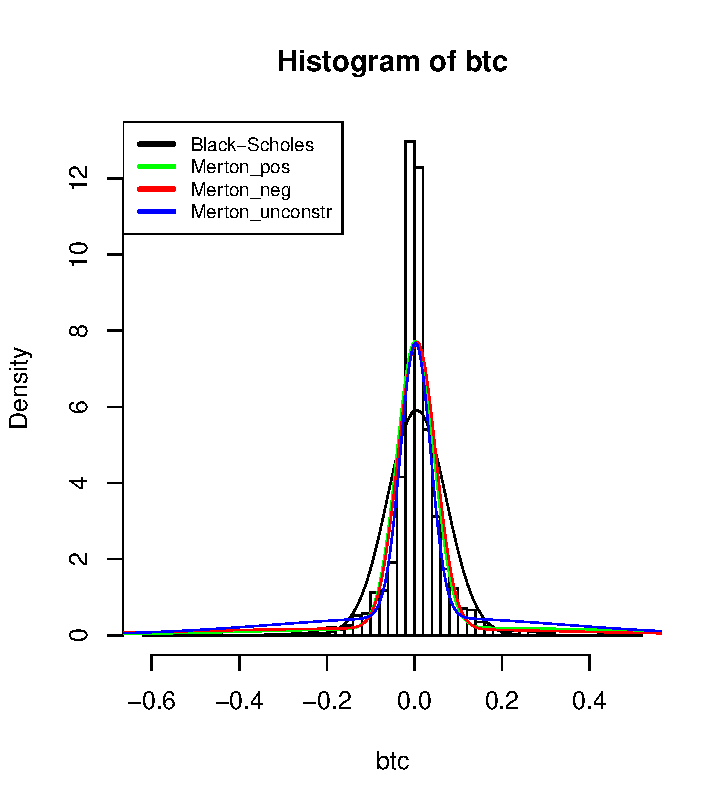
\includegraphics[width=0.8\textwidth]{historgram_10percent.pdf}
%\label{roll_stocks}
%\end{figure}
%\end{frame}

\subsection{Calibration Results}

\begin{frame}{Parameter Results}
\SmallerFont

\begin{table}[]
\begin{tabular}{llllllll}
\toprule
 & btc & bric & sp500 & eurostoxx & nasdaq & gold & wti \\
\midrule
$\mu$ & 1.497 & 0.012 & 0.128 & 0.050 & 0.183 & 0.042 & -0.038 \\
$\theta $& -0.100 & -0.100 & -0.100 & -0.100 & -0.100 & -0.100 & -0.100 \\
$\delta$ & 0.171 & 0.087 & 0.097 & 0.092 & 0.089 & 0.094 & 0.126 \\
$\lambda$ & 46.957 & 0.971 & 2.491 & 1.358 & 2.209 & 2.500 & 3.612 \\
\bottomrule
\end{tabular}
\end{table}

\begin{table}[]
\begin{tabular}{lllllll}
\toprule
 & grain & metal & eur & gbp & chf & jpy \\
\midrule
$\mu$ & -0.046 & -0.019 & -0.017 & -0.014 & 0.000 & -0.017 \\
$\theta$ & -0.100 & -0.100 & -0.100 & -0.100 & -0.100 & -0.100 \\
$\delta$ & 0.106 & 0.098 & 1.501 & 0.100 & 0.115 & 0.096 \\
$\lambda$ & 2.582 & 0.785 & 0.319 & 0.820 & 1.815 & 1.982 \\
\bottomrule
\end{tabular}

\end{table} 

\begin{table}[]
\begin{tabular}{lllll}
\toprule
 & bond\_europe & bond\_us & bond\_eur & vix \\
\midrule
$\mu $& 0.042 & 0.024 & 0.036 & -0.480 \\
$\theta $& -0.100 & -0.100 & -0.100 & -0.100 \\
$\delta$ & 0.091 & 0.099 & 0.099 & 0.236 \\
$\lambda $& 0.611 & 0.572 & 1.002 & 10.635 \\
\bottomrule
\end{tabular}
\end{table} 

\hfill All parameters are annualized.
\end{frame}

\begin{frame}{ Mean Return Comparison}
\SmallerFont
\begin{table}[]
\begin{tabular}{lllllll}
\toprule
Asset & btc & bric & sp500 & eurostoxx & nasdaq & gold \\
\midrule
Sample & 1.331 & -0.010 & 0.111 & 0.024 & 0.143 & 0.004 \\
Model & 1.497 & 0.012 & 0.128 & 0.050 & 0.183 & 0.042 \\
\bottomrule
\end{tabular}
\end{table}

\begin{table}[]
\begin{tabular}{lllllll}
\toprule
Asset & wti & grain & metal & eur & gbp & chf \\
\midrule
Sample & -0.022 & -0.062 & -0.028 & -0.013 & -0.018 & 0.006 \\
Model & -0.038 & -0.046 & -0.019 & -0.017 & -0.014 & 0.000 \\
\bottomrule
\end{tabular}
\end{table}

\begin{table}[]
\begin{tabular}{llllll}
\toprule
Asset & jpy & bond\_europe & bond\_us & bond\_eur & vix \\
\midrule
Sample & -0.030 & 0.036 & 0.024 & 0.035 & -0.034 \\
Model & -0.017 & 0.042 & 0.024 & 0.036 & -0.480 \\
\bottomrule
\end{tabular}

\end{table}
\end{frame}



\section{Correlation}
\subsection{Correlation Results}

\begin{frame}{Bitcoin Correlation Comparison}
\SmallerFont
\begin{table}[]
\begin{tabular}{llllll}
\toprule
 & bric & sp500 & eurostoxx & nasdaq & gold \\
 \midrule
Sample & -0.0134 & -0.0123 & 0.0320 & -0.0119 & -0.0063 \\
Model & 0.0141 & 0.0437 & 0.0368 & 0.0359 & -0.0024 \\
\bottomrule
\end{tabular}
\end{table}

\begin{table}[]
\begin{tabular}{lllllll}
\toprule
 & wti & grain & metal & eur & gbp & chf \\
 \midrule
Sample & 0.0232 & 0.0234 & 0.0072 & 0.0268 & 0.0182 & 0.0210 \\
Model & 0.0077 & 0.0350 & 0.0269 & 0.0229 & 0.0073 & 0.0246 \\
\bottomrule
\end{tabular}
\end{table}

\begin{table}[]
\begin{tabular}{llllll}
\toprule
 & jpy & bond\_europe & bond\_us & bond\_eur & vix \\
 \midrule
Sample & -0.0123 & -0.0132 & -0.0216 & -0.0075 & 0.0182 \\
Model & -0.0109 & -0.0238 & -0.0184 & -0.0098 & -0.0509 \\
\bottomrule
\end{tabular}
\end{table}

\end{frame}


\begin{frame}{Correlation Comparison}
\begin{figure}
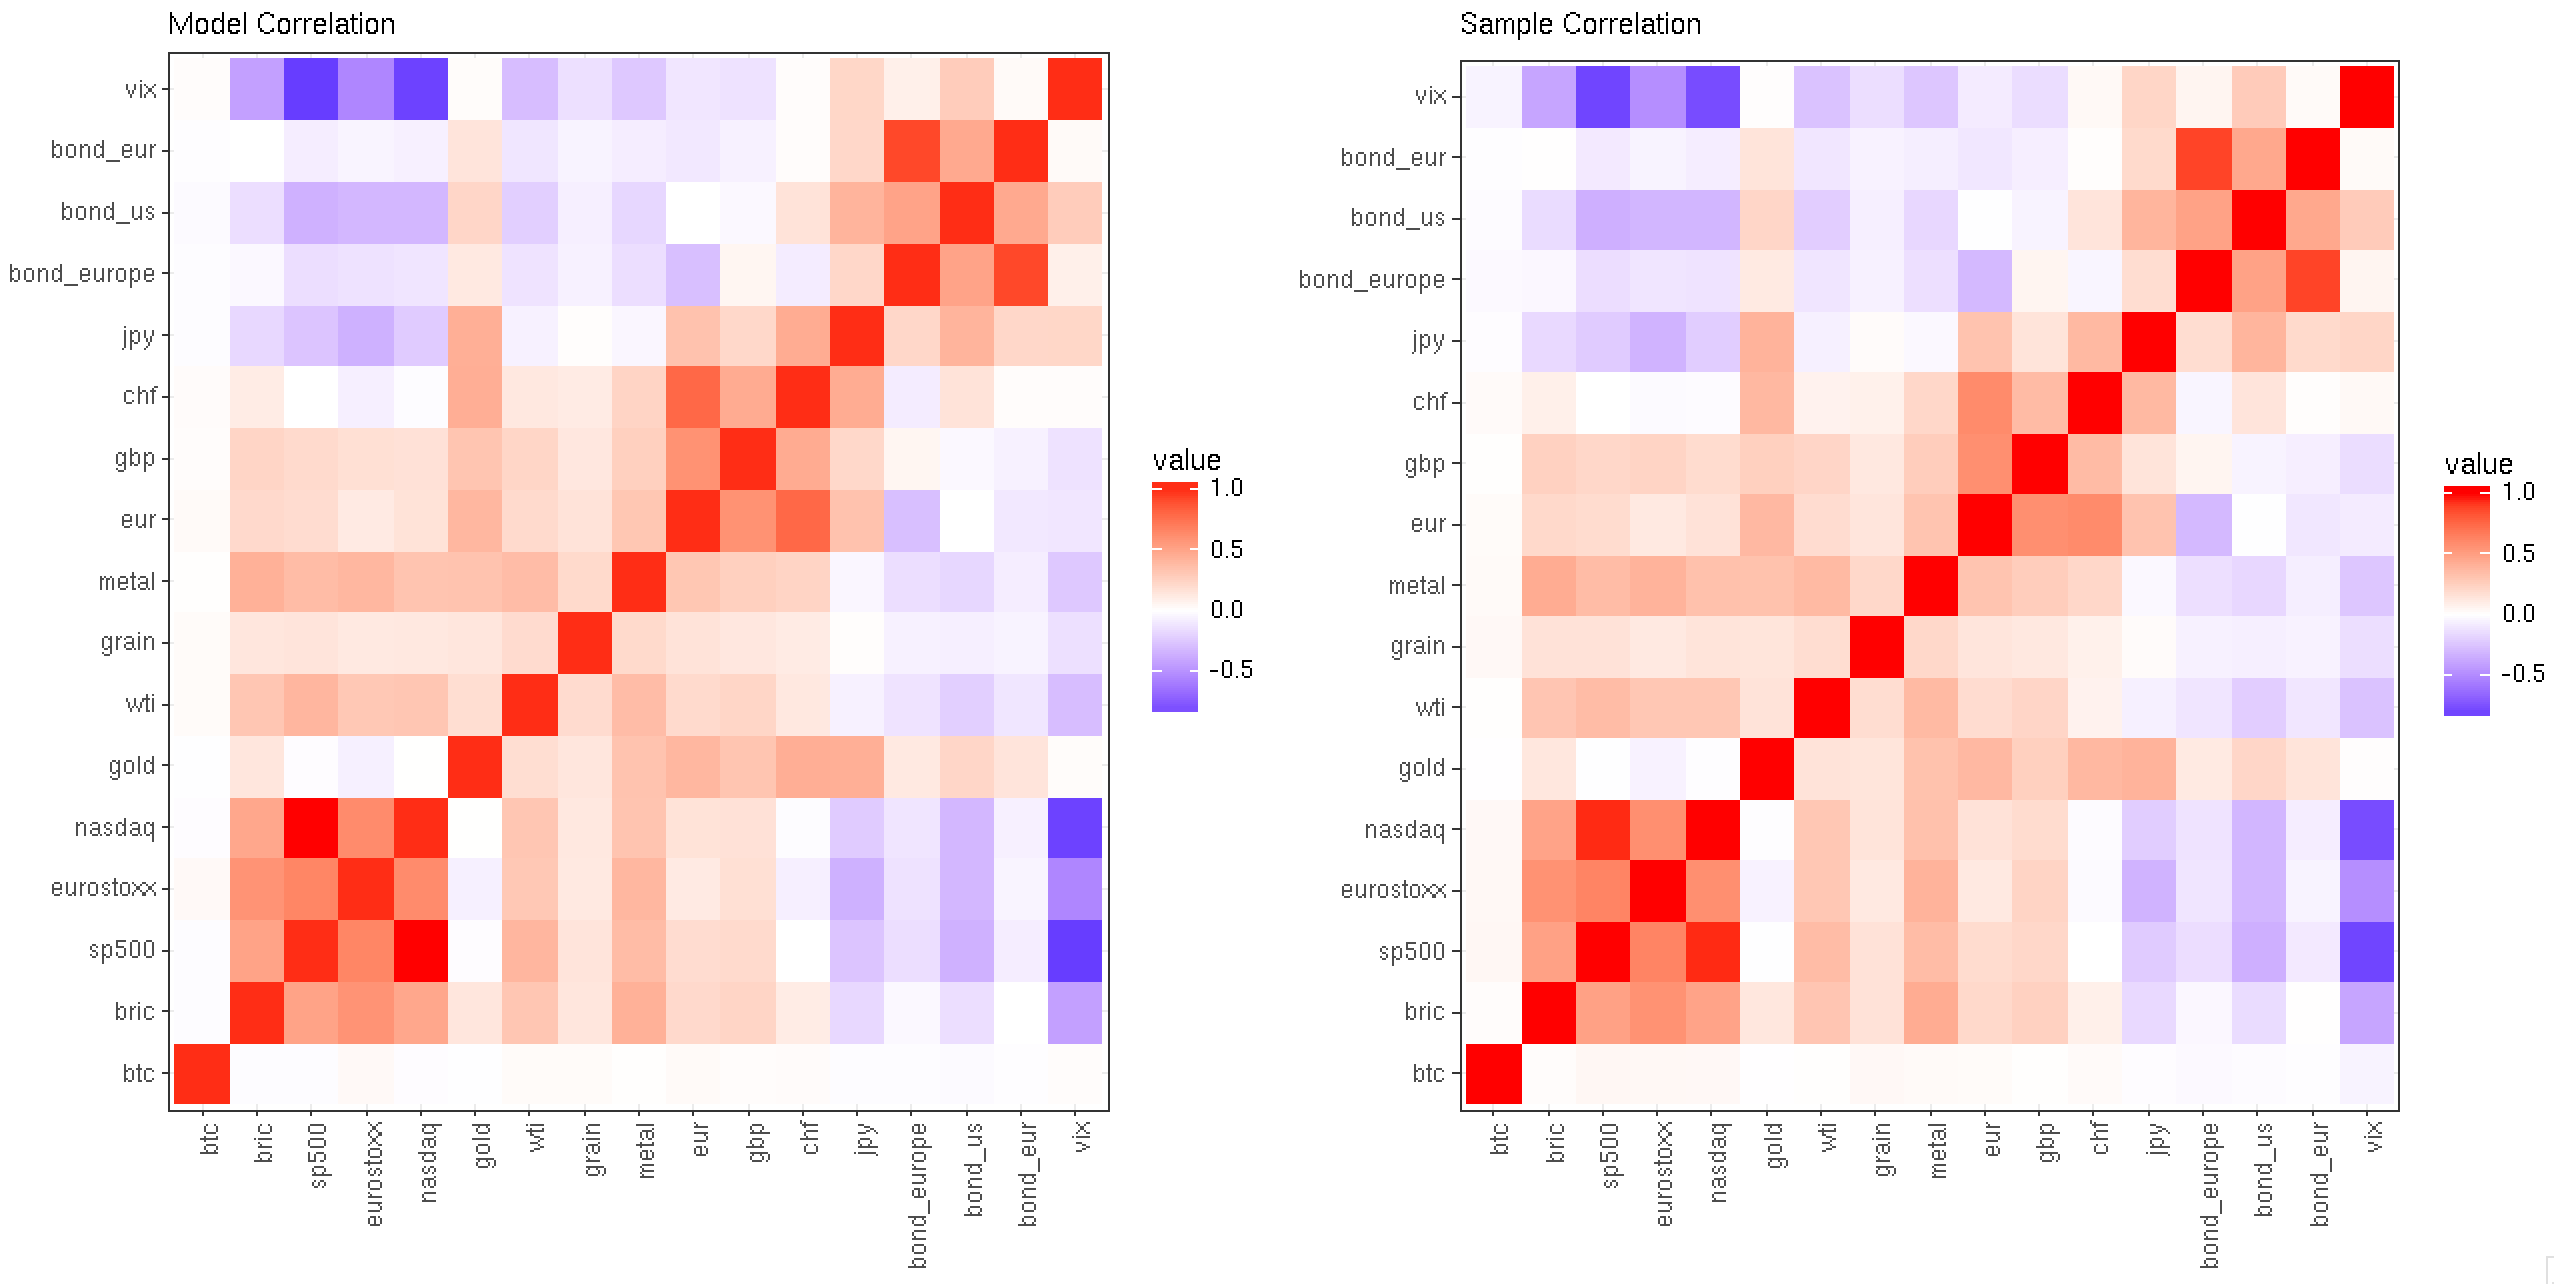
\includegraphics[width=\textwidth]{correlation_comparison}
\caption{The calibrated model is able to reproduce the correlation structure in the dataset very closely.}
\end{figure}
\end{frame}

\subsection{Correlation Significance}

\begin{frame}{Tests on Correlation Significance}
\small
We perform two different tests of the type:
\begin{equation*}
H_0 : \rho= 0 \quad vs  \quad H_1 : \rho \neq 0
\end{equation*} 

for the empirical correlation between Bitcoin and the other assets computed as Pearson's sample correlation:
\begin{equation*}
r_{X,Y} = \frac{\sum_{i = 1}^{N} (x_i - \bar{x})(y_i - \bar{y})}{\sqrt{\sum_{i = 1}^{N} (x_i - \bar{x})^2 \sum_{i = 1}^{N} (y_i - \bar{y})^2}}
\end{equation*}

Pearson's test is a simple t-test, the downside is that the underlying hypotheses are normality of both samples but also works if samples are large  enough.
Permutation test is a more general test with no additional hypotheses but is performed through simulation.

We report the \textit{p-value} for all tests. Considering a confidence level of $5\%$, whenever a \textbf{p-value is higher than $\mathbf{0.05}$} the test is telling us that \textbf{there is no statistical evidence} allowing us  \textbf{to assert that the correlation is different from zero}.

\end{frame}


\begin{frame}{Correlation Significance with Bitcoin}
\SmallerFont
\begin{table}[]
\begin{tabular}{lllllll}
\toprule
 & bric & sp500 & eurostoxx & nasdaq & gold & wti \\
\midrule
Correlation & 0.0141 & 0.0437 & 0.0368 & 0.0359 & -0.0024 & 0.0077 \\
Pearson & 0.504 & 0.044 & 0.094 & 0.089 & 0.905 & 0.719 \\
Permutation & 0.512 & 0.042 & 0.087 & 0.095 & 0.911 & 0.720 \\
Spearman & 0.922 & 0.459 & 0.157 & 0.329 & 0.423 & 0.459 \\
\bottomrule
\end{tabular}
\end{table}

\begin{table}[]
\begin{tabular}{lllllll}
\toprule
 & grain & metal & eur & gbp & chf & jpy \\
\midrule
Correlation & 0.0350 & 0.0269 & 0.0229 & 0.0073 & 0.0246 & -0.0109 \\
Pearson & 0.108 & 0.195 & 0.291 & 0.747 & 0.239 & 0.608 \\
Permutation & 0.103 & 0.211 & 0.286 & 0.733 & 0.253 & 0.613 \\
Spearman & 0.170 & 0.798 & 0.453 & 0.697 & 0.905 & 0.474 \\
\bottomrule
\end{tabular}

\end{table}

\begin{table}[]
\begin{tabular}{lllll}

\toprule
 & bond\_europe & bond\_us & bond\_eur & vix \\
\midrule
Correlation & -0.0238 & -0.0184 & -0.0098 & -0.0509 \\
Pearson & 0.285 & 0.408 & 0.642 & 0.018 \\
Permutation & 0.268 & 0.393 & 0.649 & 0.018 \\
Spearman & 0.468 & 0.336 & 0.816 & 0.330 \\
\bottomrule
\end{tabular}
\end{table}

Values reported are the \textit{p-values} for three test on $H_0: \rho=0$ vs $H_1: \rho \neq 0$.
\end{frame}


\subsection{Rolling Correlation}

\begin{frame}{Rolling Correlation between Bitcoin and Stocks}
\begin{figure}
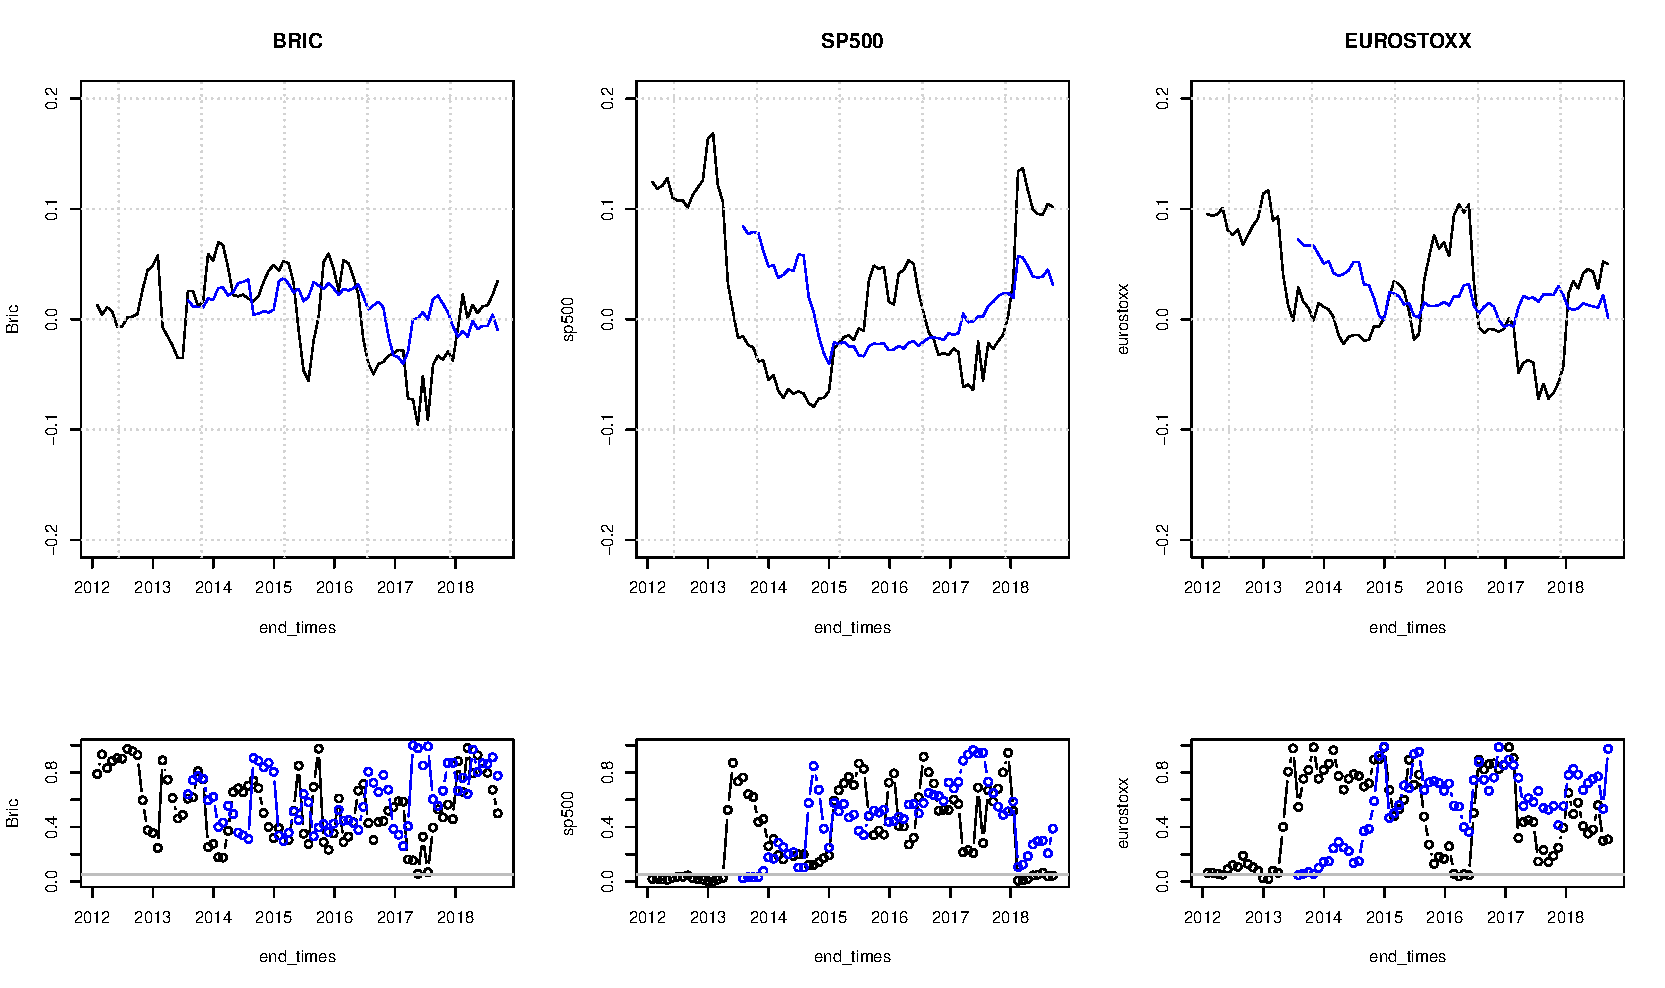
\includegraphics[width=\textwidth]{rolling_stocks.pdf}
\label{roll_stocks}
\caption{In blue we have the 3 year rolling correlation, in black the 18 month rolling correlation, both updated monthly.}
\end{figure}
\end{frame}

\begin{frame}{Rolling Correlation between Bitcoin and Bonds and VIX}
\begin{figure}
	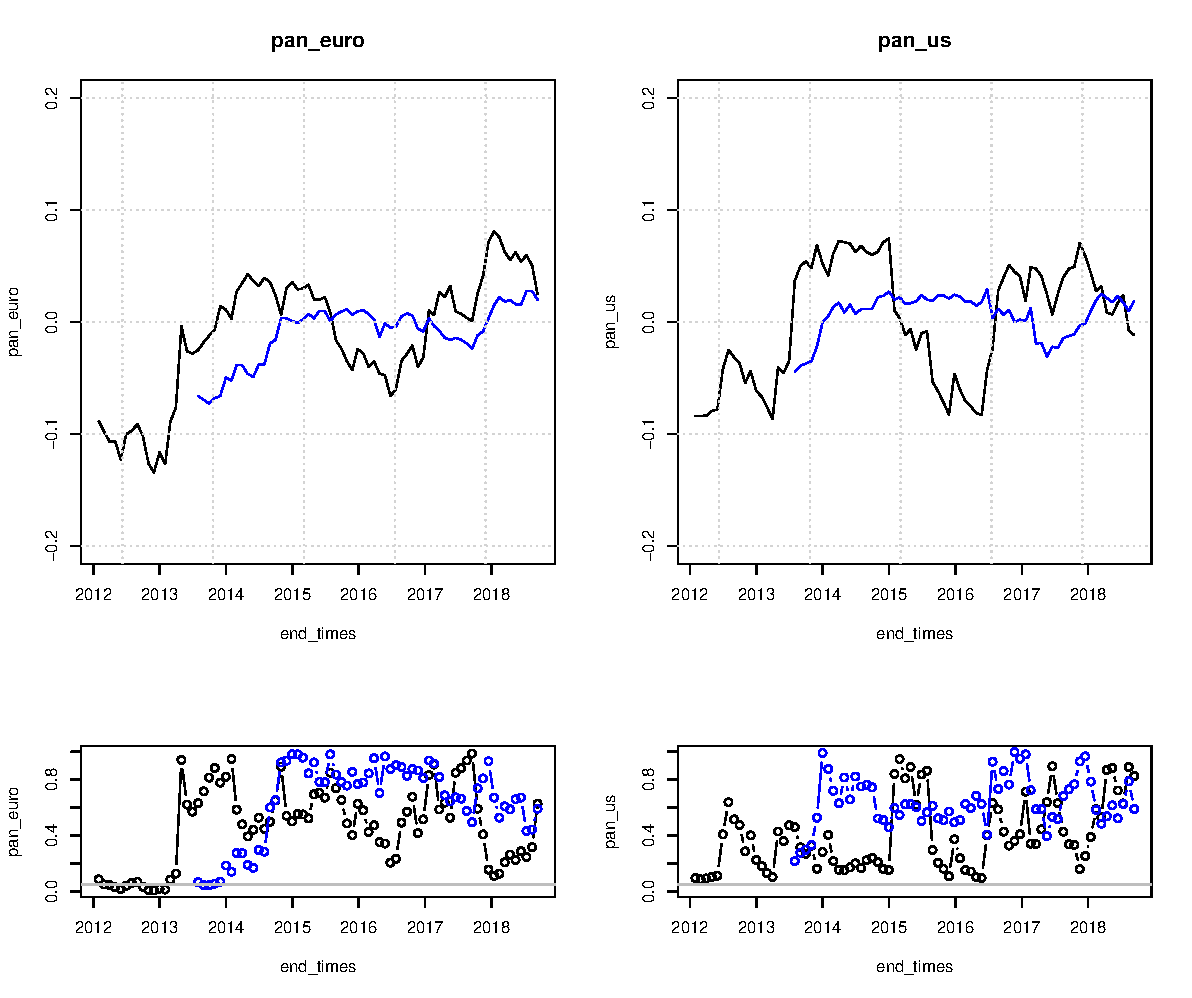
\includegraphics[width=\textwidth]{rolling_bonds.pdf}
	\label{roll_bonds}
	\caption{In blue we have the 3 year rolling correlation, in black the 18 month rolling correlation, both updated monthly.}
\end{figure}
\end{frame}

\begin{frame}{Rolling Correlation between Bitcoin and Currencies}
\begin{figure}
	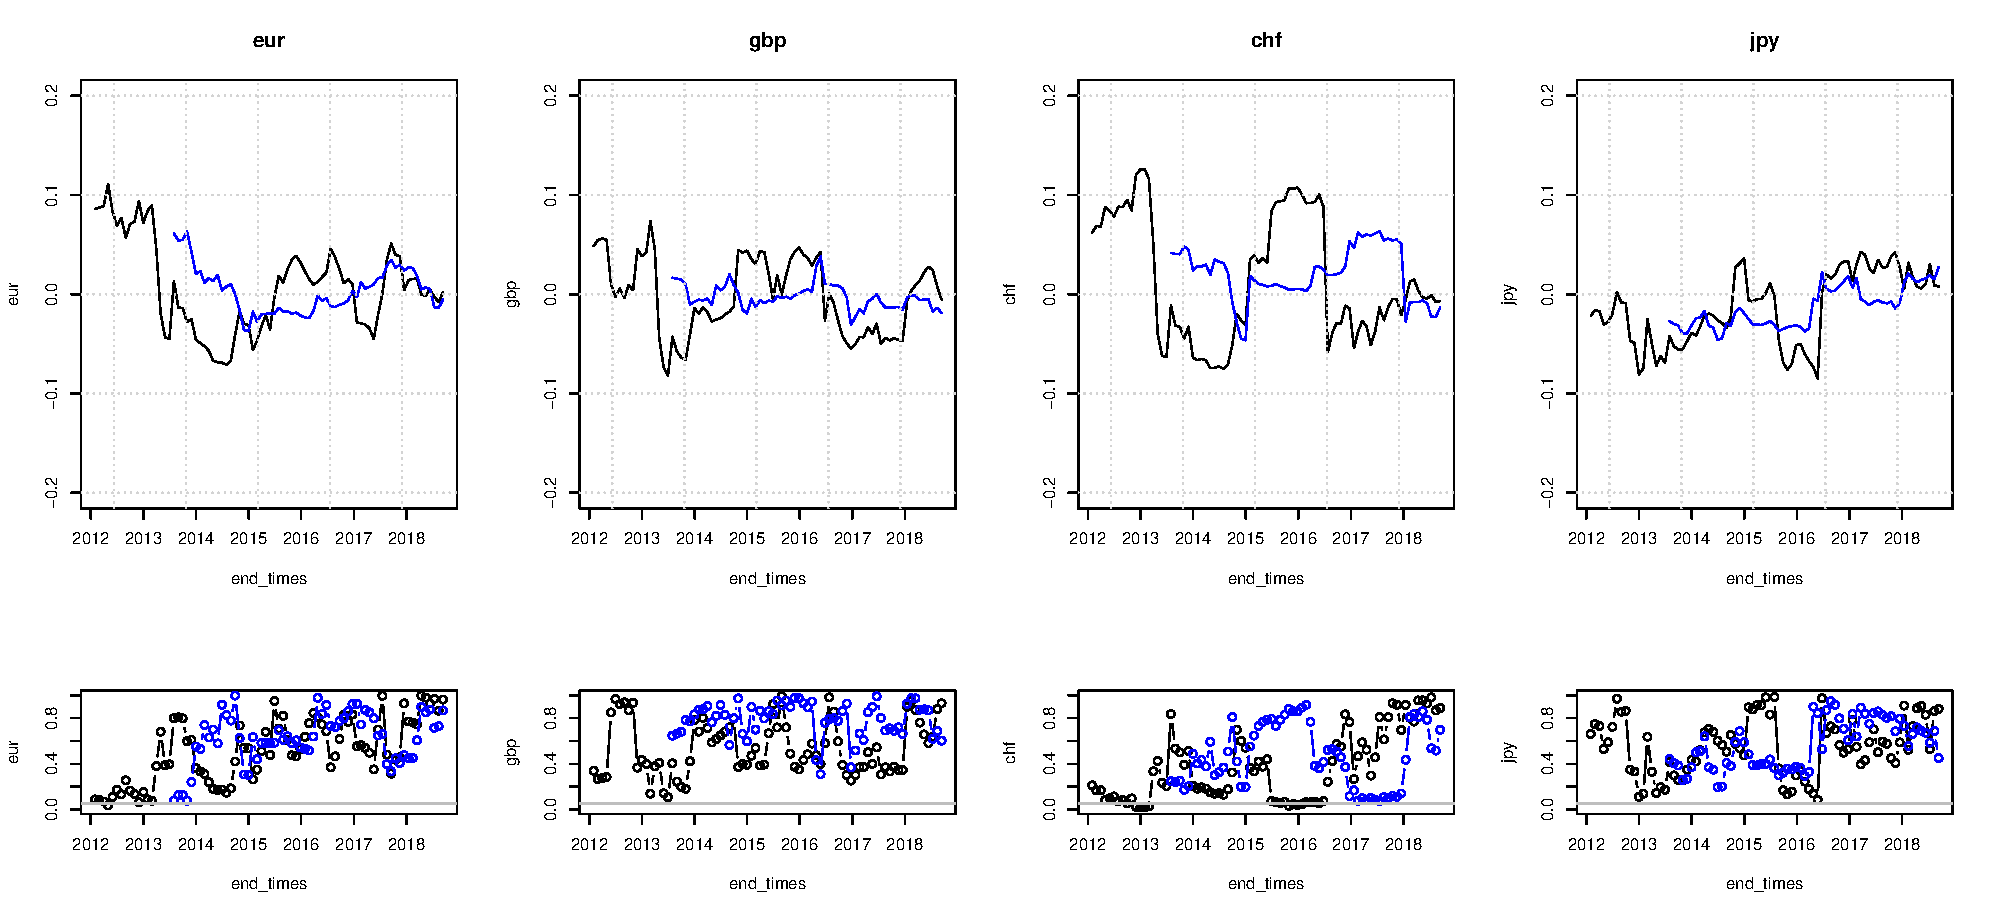
\includegraphics[width=\textwidth]{rolling_fx.pdf}
	\label{roll_fx}
	\caption{In blue we have the 3 year rolling correlation, in black the 18 month rolling correlation, both updated monthly.}
\end{figure}
\end{frame}

\begin{frame}{Rolling Correlation between Bitcoin and Commodities}
\begin{figure}
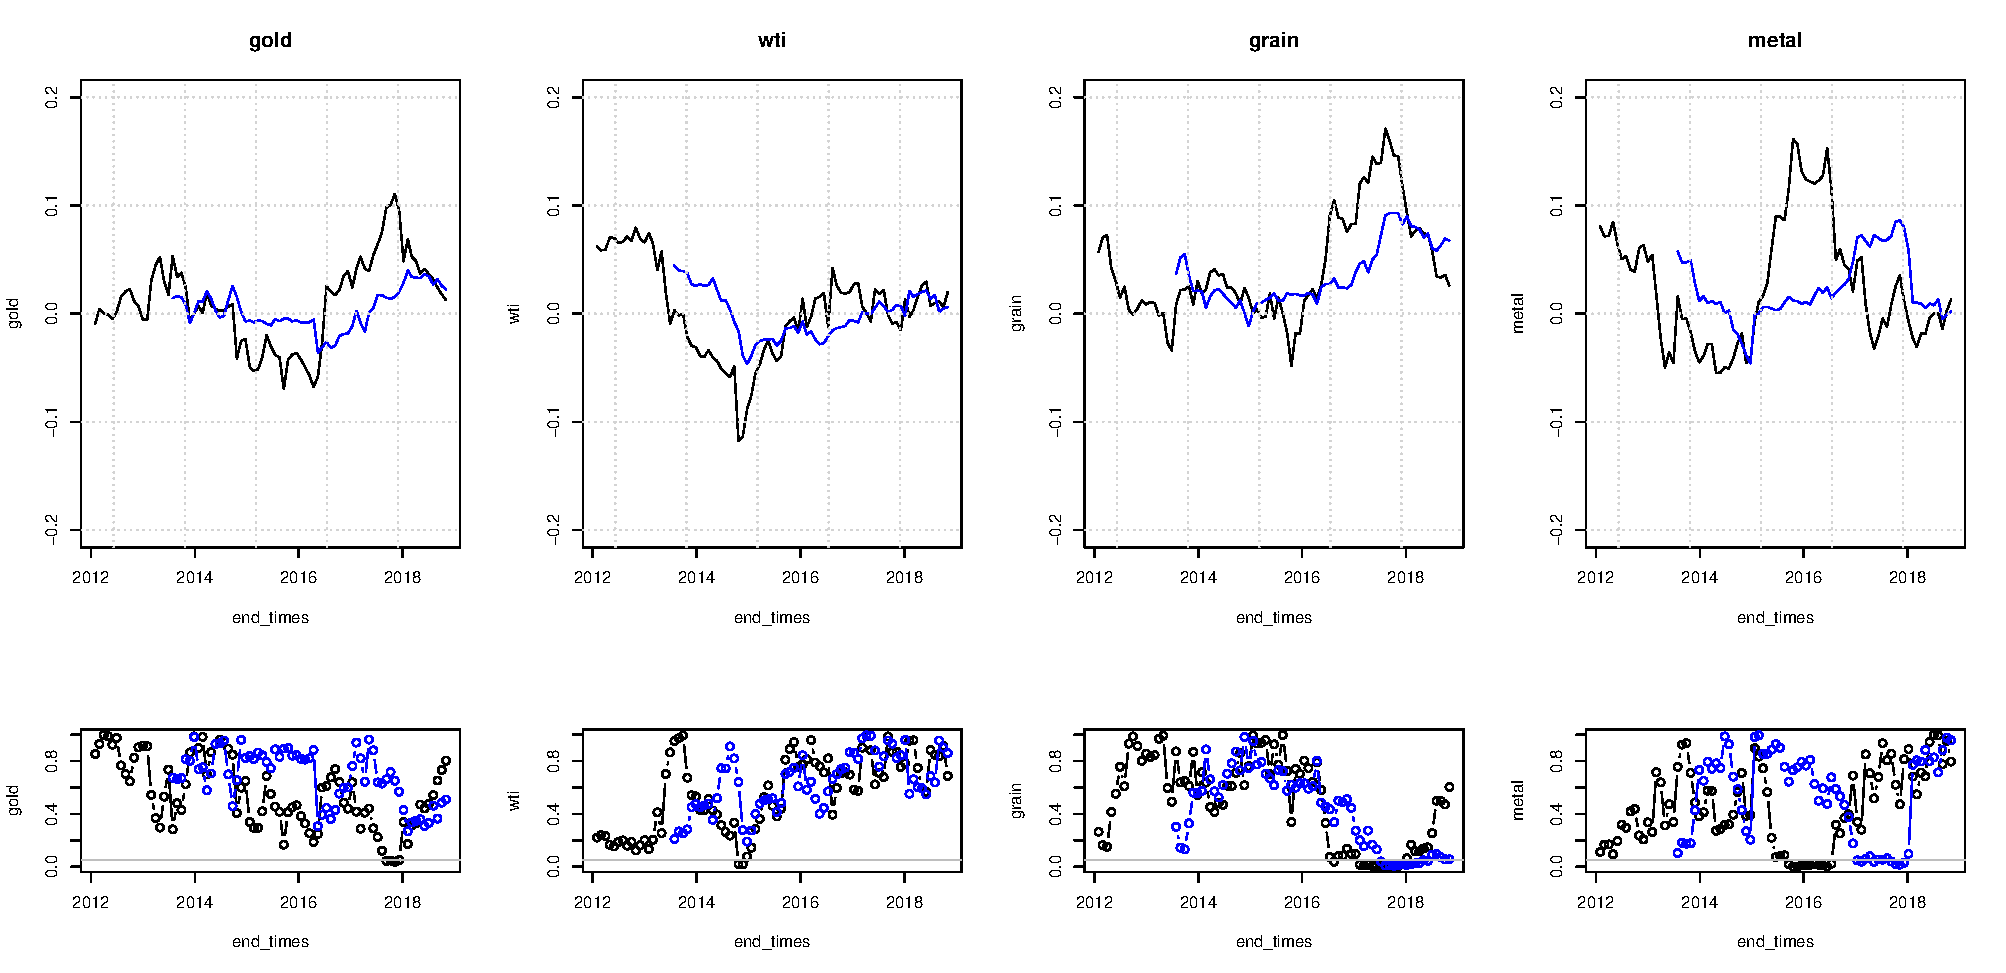
\includegraphics[width=\textwidth]{rolling_commodities.pdf}
\label{roll_comm}
\caption{In blue we have the 3 year rolling correlation, in black the 18 month rolling correlation, both updated monthly.}
\end{figure}
\end{frame}



\section{Efficient Frontier}

\begin{frame}{Efficient  Frontier and Optimal Allocation}
The two approaches considered both involve the minimization of a \textit{risk measure} given a level of target returns:
\begin{itemize}
	\item \textit{Markowitz Mean-Variance optimization}:  minimize the portfolio variance (or equivalently the volatility) as originally proposed in \cite{MARKOWITZ}. This approach has explicit formulas for the solution in the unconstrained case.
	\item \textit{CVaR optimization}: minimize the portfolio \textit{conditional VaR} rather than the simple VaR due to the mathematical properties of the former (CVaR is a coherent risk measure). Numerical algorithms are required.
\end{itemize}
\end{frame}


\begin{frame}{Efficient  Frontier and Optimal Allocation}
\begin{subequations}
	\begin{align}
	&\!\min_{\mathbf{w}\in \mathbb{R}^{n}}        & & PtfRisk(\mathbf{w}) \notag\\
	& \text{subject to} &      & \mathbf{e}'\mathbf{w} = 1 , \notag\\
	&                  &      & \mathbf{r}'\mathbf{w} = r_{target},\label{eq:constraint2} \notag\\
	&		 &        & w_{i} \geq 0, \text{for} \: i = 1\dots n. \notag
	\end{align}
\end{subequations}

where:
\begin{itemize}
	\item \textbf{w} is the vector of weights,
	\item \textbf{r} is the vector of returns,
	\item \textbf{e} indicates a vector of ones,
	\item $r_{target}$ is the target portfolio return,
	\item the last constraint is included only when shortselling is not allowed.
\end{itemize}

In the Markowitz case the risk measure is the portfolio variance $\mathbf{w}'\Sigma \mathbf{w}$, in the CVaR case is the portfolio CVaR at level $95\%$.
\end{frame}

\subsection{Markowitz Efficient Frontier}

\begin{frame}{Markowitz Efficient Frontier}
\begin{figure}
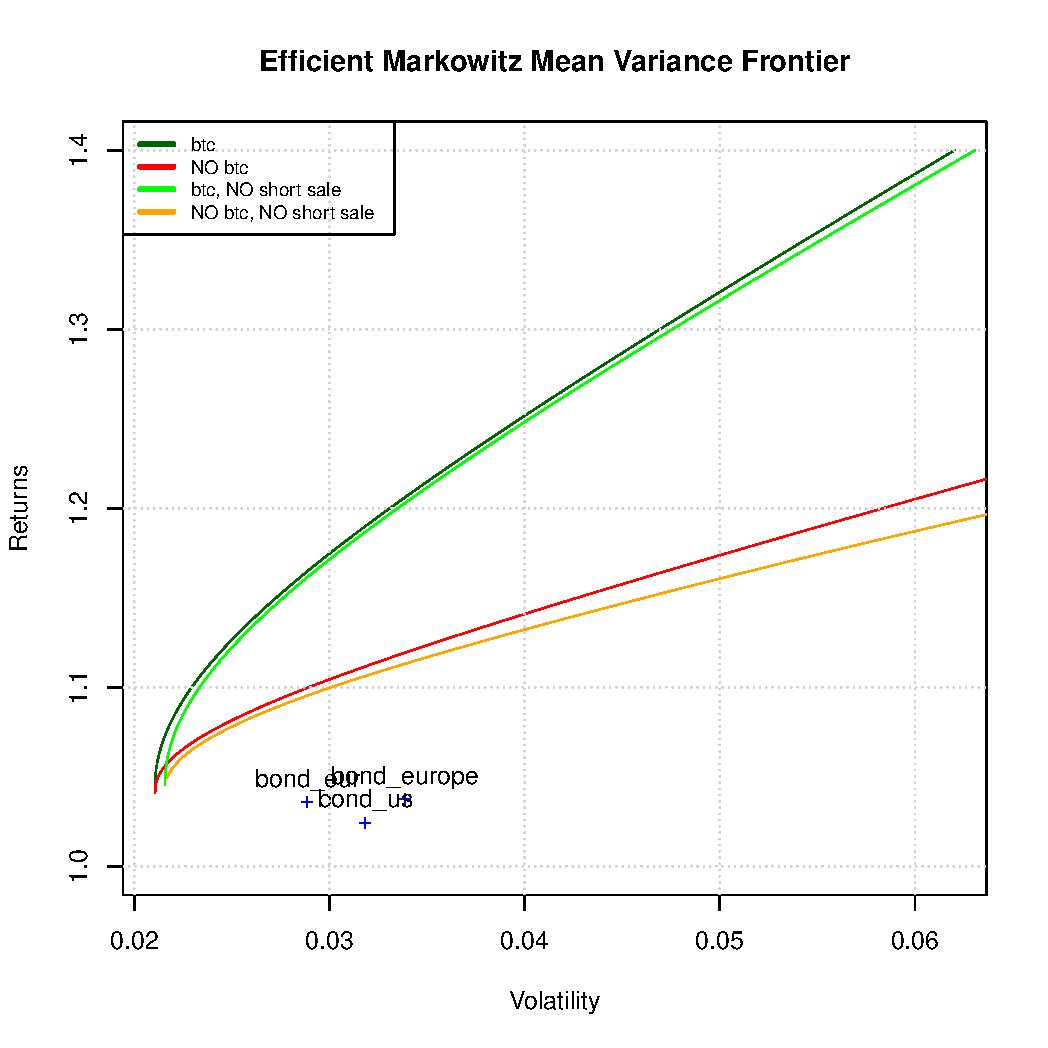
\includegraphics[width=0.65\textwidth]{frontier_markowitz_sample_percentage.pdf}
\caption{Efficient frontier for the sample percentage returns We can see how including Bitcoin effectively diversifies the portfolio.}
\end{figure}
\end{frame}

\begin{frame}{Markowitz allocation including Bitcoin}
\begin{figure}
	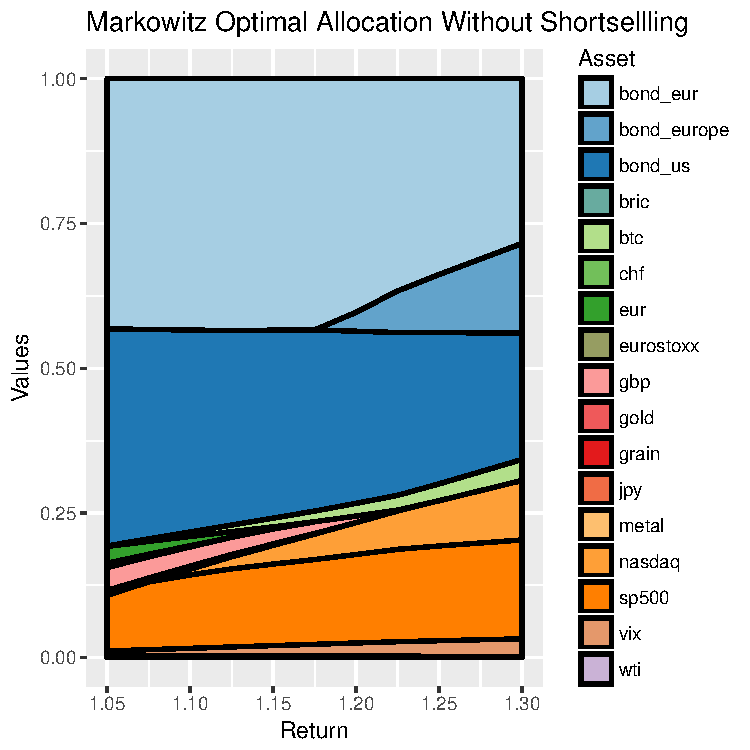
\includegraphics[width=0.5\textwidth]{allocation_sample_btc_percentage}
	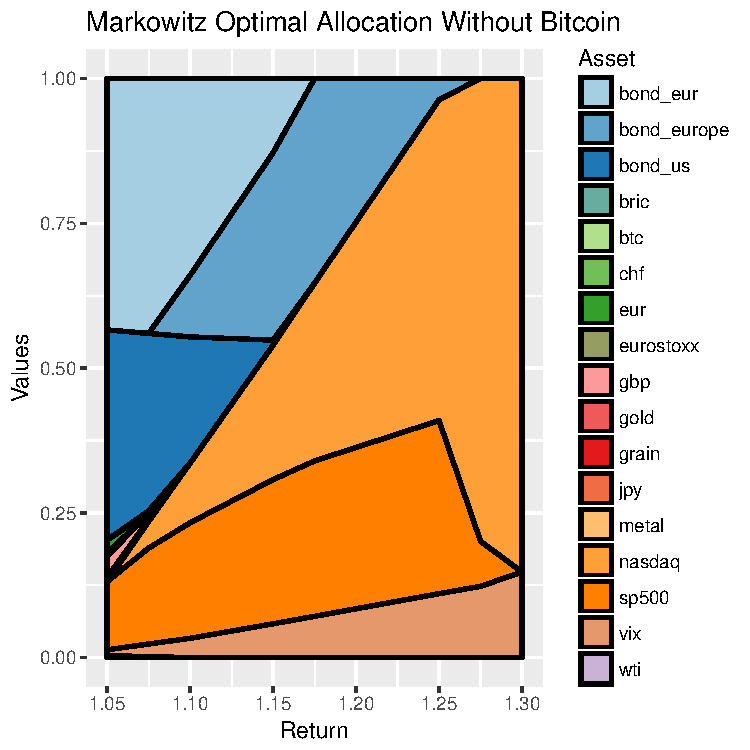
\includegraphics[width=0.5\textwidth]{allocation_sample_nobtc_percentage}
	\caption{We can see in green that the allocation in Bitcoin is about $3\%$ and increases with the target return.}
\end{figure}
\end{frame}

\subsection{CVaR Efficient Frontier}
\begin{frame}{CVaR Efficient Frontier}
Since we only have the empirical distribution of the returns, we have to compute the CVaR empirically as well. We considered two approaches: 

\begin{enumerate}
	\item \textit{Annual returns simulation}: given the set of all available daily returns, extract 255 of them to simulate one annual return scenario. Repeat to get a number of simulations (in our case 10,000).
	We will refer to this method as annual bootstrap.
	\item \textit{Daily return as scenarios}: consider the latest $N = 255 * 5 = 1275$  daily return and use them as the different scenario realizations.
\end{enumerate}
\end{frame}

\begin{frame}{CVaR Efficient Frontier (annual bootstrap)}
\begin{figure}
	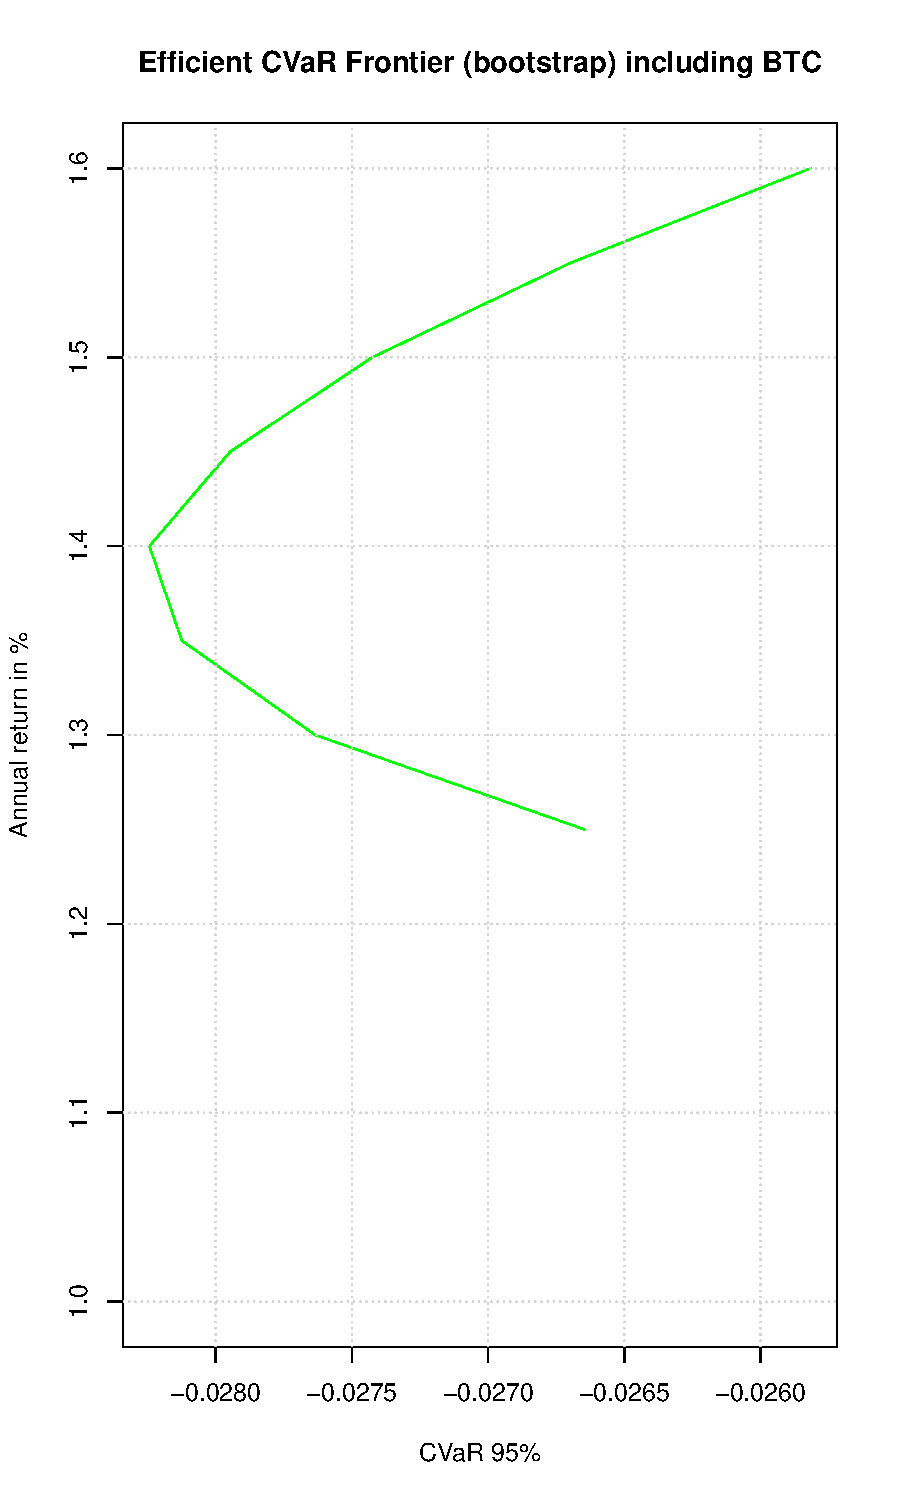
\includegraphics[width=0.4\textwidth]{frontier_bootstrap_btc.pdf}
	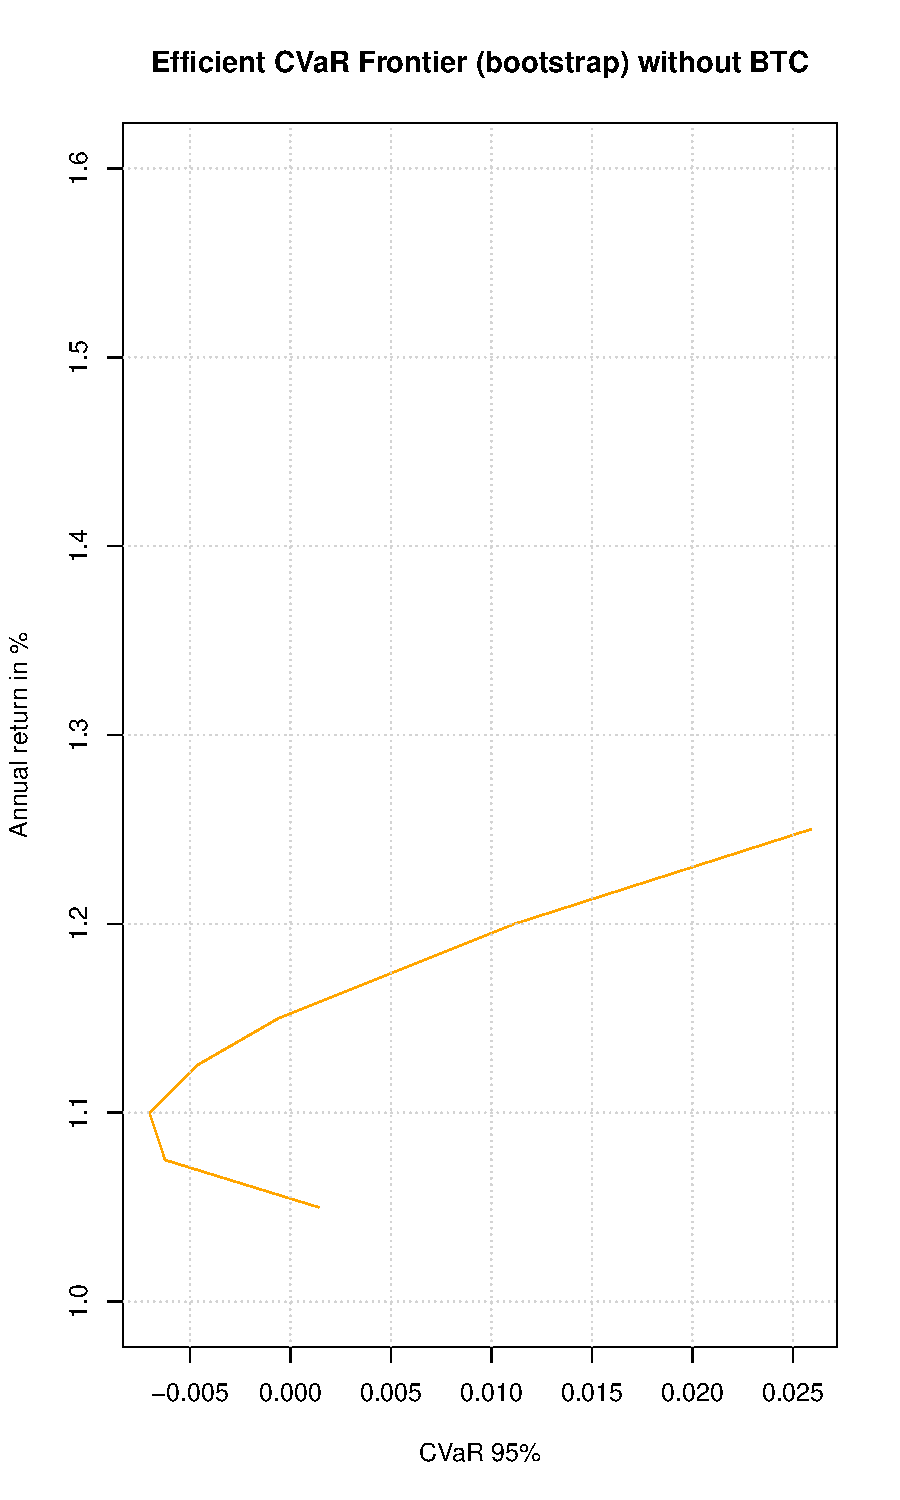
\includegraphics[width=0.4\textwidth]{frontier_bootstrap_nobtc.pdf}

\end{figure}
\end{frame}

\begin{frame}{Optimal Allocation (annual bootstrap)}
\begin{figure}
	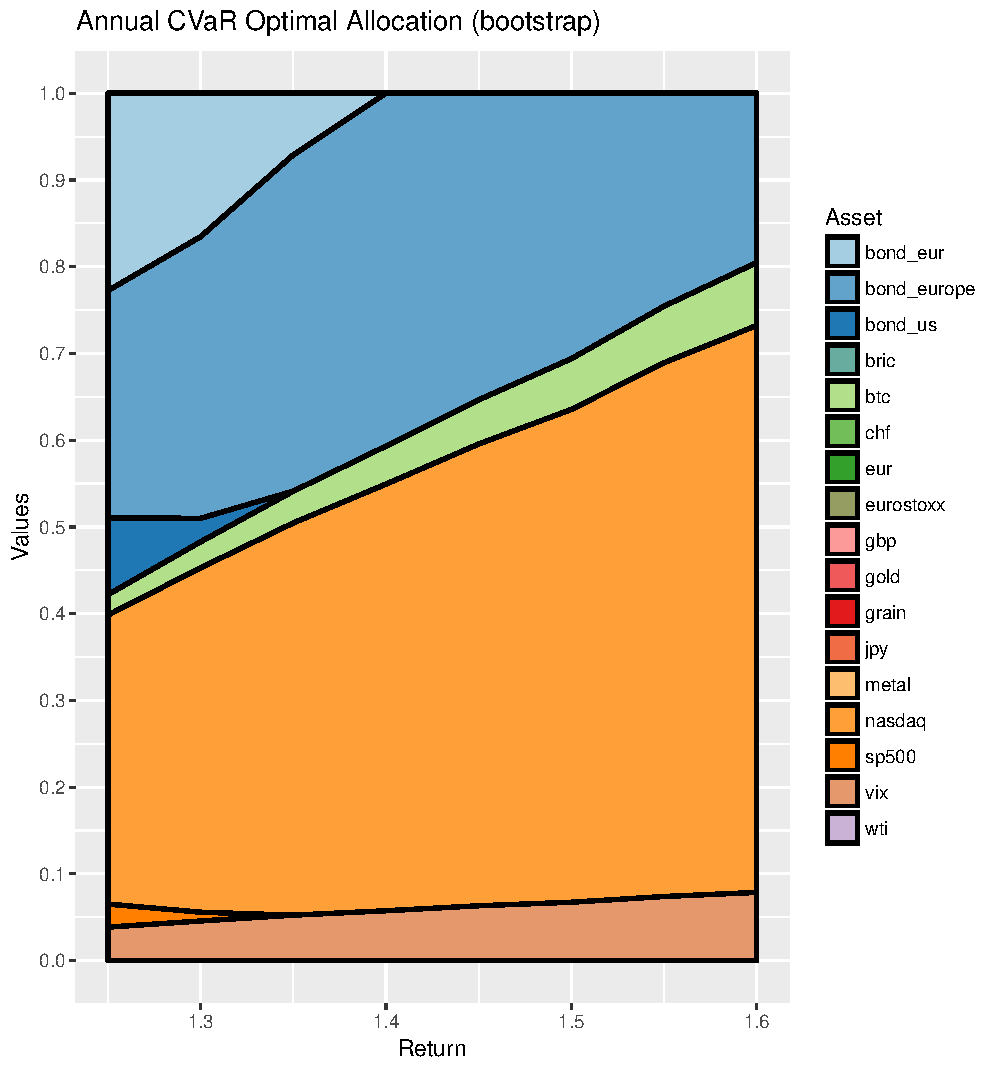
\includegraphics[width=0.5\textwidth]{allocation_bootstrap_btc.pdf}
	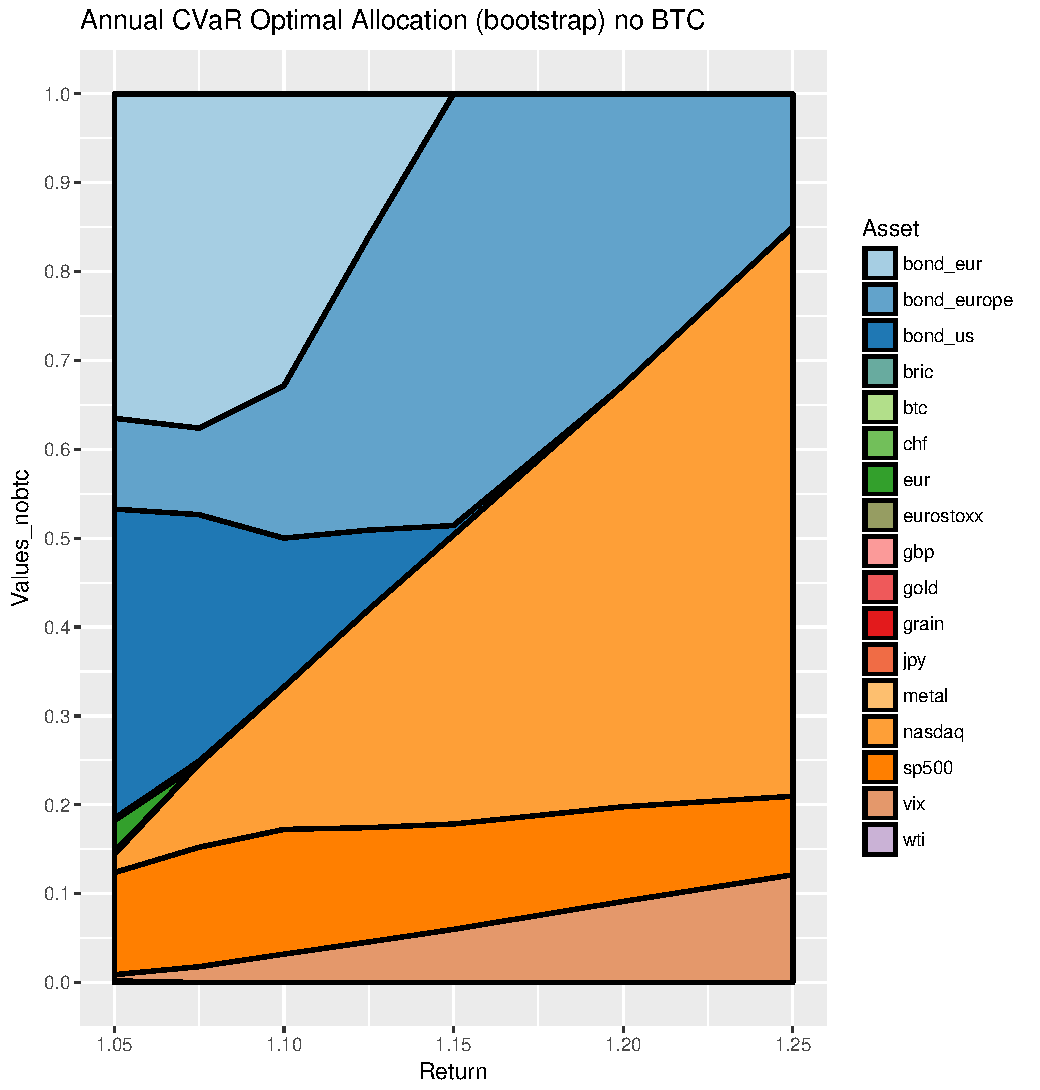
\includegraphics[width=0.5\textwidth]{allocation_bootstrap_nobtc.pdf}
\end{figure}
\end{frame}

\begin{frame}{CVaR Efficient Frontier (daily returns)}
\begin{figure}
	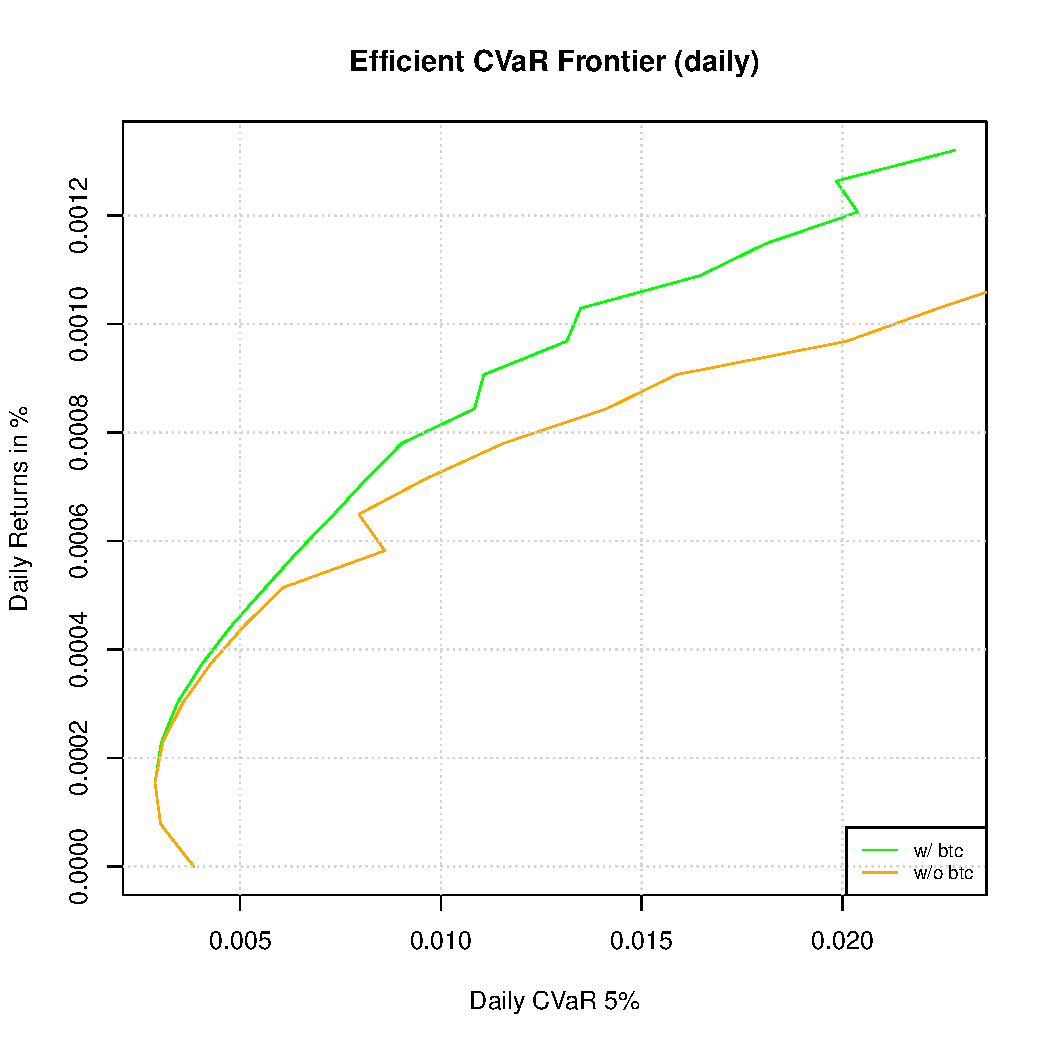
\includegraphics[height= 0.8\textheight]{frontier_daily.pdf}
\end{figure}
\end{frame}

\begin{frame}{Optimal Allocation (daily returns)}
\begin{figure}
	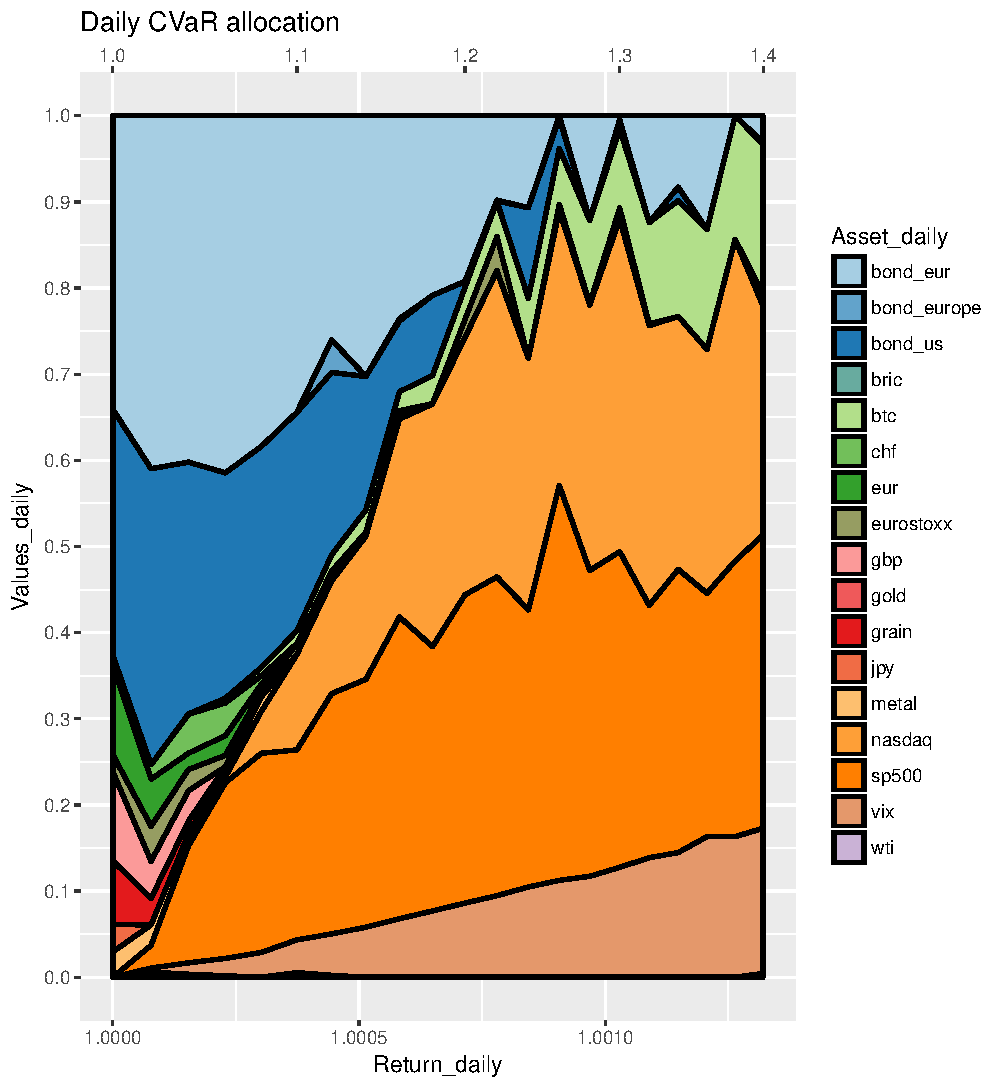
\includegraphics[width=0.5\textwidth]{allocation_daily_btc.pdf}
	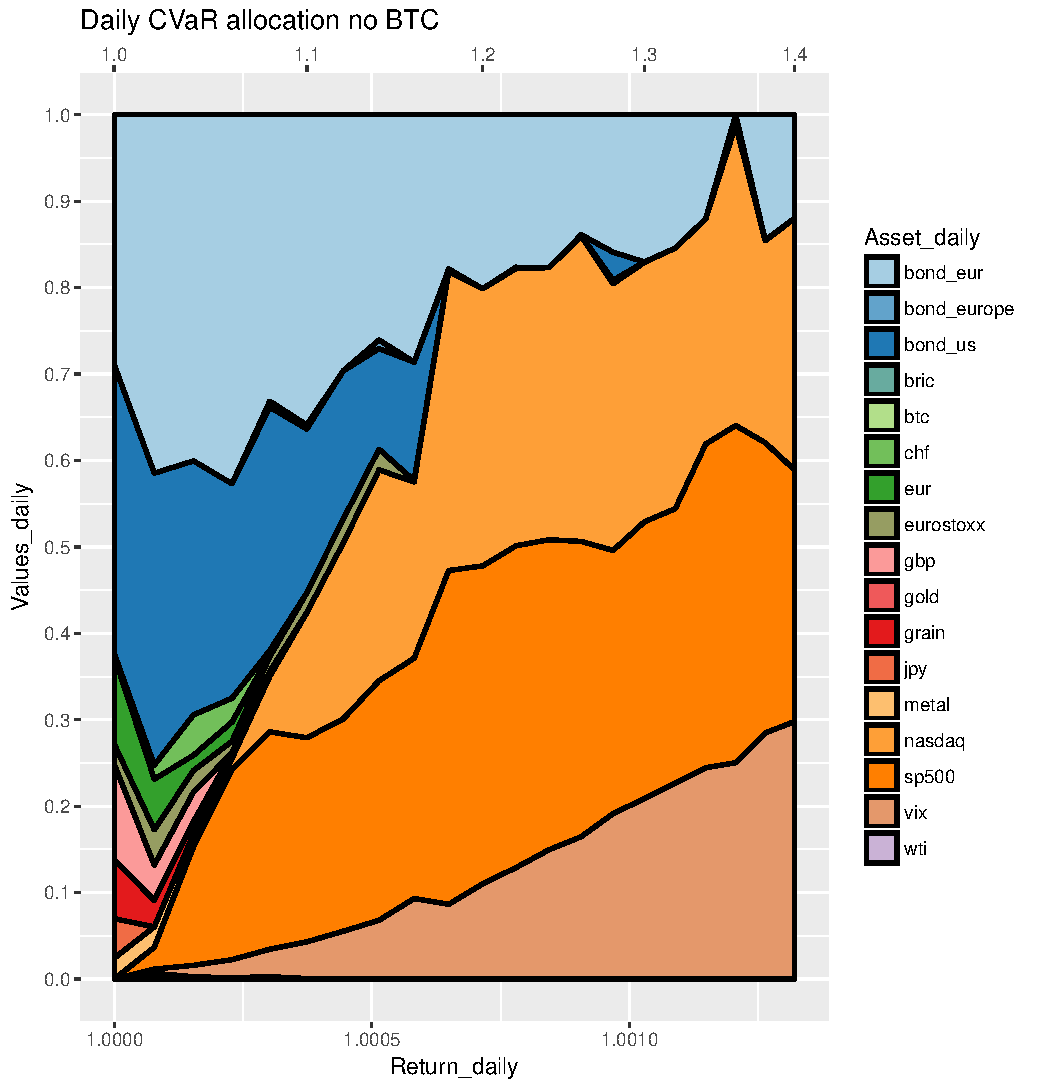
\includegraphics[width=0.5\textwidth]{allocation_daily_nobtc.pdf}
\end{figure}
\end{frame}

\begin{frame}[allowframebreaks] %allow to expand references to multiple frames (slides)
\frametitle{References}

\scriptsize{\bibliographystyle{acm}}

\bibliography{my_bibliography} %bibtex file name without .bib extension

\end{frame}

\end{document}

